\chapter{Travail réalisé}


\section{Aperçu général}
Voici la chronologie du travail réalisé en entreprise.\\
\ganttset{%
	calendar week text={%
		\pgfcalendarmonthshortname{\startmonth}~\startday%
	}%
}
\newganttlinktype{f-m}{
	\ganttsetstartanchor{on right=1}
	\ganttsetendanchor{on left=0}
	\draw[/pgfgantt/link]
	([xshift=-.2pt]\xLeft, \yUpper) --       % xshift to fit arrow
	node[pos=.5, /pgfgantt/link label node] {\ganttlinklabel} 
	(\xRight, \yLower);
}


%vgrid={*1{blue!30},
%	*6{black,dotted},
%	*1{red!30},
%	*2{black,dotted},
%	*1{blue!30},
%	*{34}{black,dotted},
%	*1{green!30},
%	*1{red!30},
%	*{10}{black,dotted},
%	*1{green!30}},
\setganttlinklabel{f-m}{}

\begin{ganttchart}[
	hgrid={*1{black!30,dotted}},
	vgrid={*1{black!30,dotted}},
	x unit=3mm,
	time slot format=isodate,
	inline,
	bar/.append style={fill=blue!37},
	bar height=.5,
	group/.append style={draw=black, fill=black!50},
	milestone/.append style={fill=green!20, rounded corners=6pt,scale=2},
	milestone inline label node/.append style={right=1mm},
	]{2019-03-28}{2019-05-25}
	\gantttitlecalendar{year, month=name, week} \\
	\ganttgroup{Analyse des besoins}{2019-03-29}{2019-04-9}\\
	\ganttgroup{Réalisation technique}{2019-04-5}{2019-05-13}\\
	\ganttgroup{Maintenance}{2019-05-13}{2019-05-24} \\
	\ganttbar[bar height=.5]{OFBiz}{2019-04-01}{2019-04-11}\\
	\ganttbar[
	bar/.append style={ fill=red!50
	}]{REST}{2019-04-08}{2019-04-28} \\
	\ganttbar[
	bar/.append style={ fill=orange!50
	}]{Entitymaint}{2019-04-20}{2019-05-12} \\

	\ganttmilestone{Preuve de concept}{2019-05-12}] \\
	\ganttbar[
	bar/.append style={ fill=purple!40, dashed
	}]{Revue de code}{2019-05-13}{2019-05-23} \\
	\ganttlink{elem3}{elem4}
	\ganttlink{elem4}{elem5}
	\ganttlink[link type=f-m]{elem5}{elem6}
	\ganttlink[link type=dr]{elem4}{elem6}
	\ganttlink[link type=f-m]{elem6}{elem7}
\end{ganttchart}

\newpage









\section{Environnement}

\subsection{Installation de l'environnement}
Avant tout, mon intégration a commencé par l'installation du poste de travail suivi par une discussion sur le choix de distribution Linux , la configuration des outils utilisés par l'entreprise ainsi que par la mise en place des accès aux ressources internes. Le choix d'IDE à été fait au faveur de IntelliJ car il possède des nombreux moyens de navigation qui sont incontournables dans la structure de OFBiz riche en dualité XML/Java. 




\subsection{Formation générale}


Lors de la formation générale, traditionnellement prévue pour tout les nouveau venus de Néréide, j'ai pu découvrir le fonctionnement basique de OFBiz à travers les démonstration des projets existants. Les points soulevés comportait la gestion des dépendances à travers \verb|Gradle| et \verb|Ant|\footnote{Ant étant déprécié depuis la version 16.11 de OFBiz mais certains projets client l'utilisent toujours car ils se basent sur une version antérieure.  }, une introduction au langage Groovy et les raisons pour lesquelles il a été préféré au DSL propre à OFBiz \footnote{Pour remplacer le DSL en XML  sous le nom Mini lang, en train d'être entièrement \href{https://cwiki.apache.org/confluence/display/OFBIZ/Mini+Lang+Deprecation}{déprécié}. }


\subsection{Jira}
Un autre point intéressant était le système de gestion de tickets \verb|Jira | utilisé par l'entreprise qui permet de suivre et gérer les bugs tout en interagissant avec les clients. L'outil est utilisé également par la plupart des projet communautaires Apache, dont OFBiz.

\subsection{Approfondissement de Git }
Même si la gestion de versions de OFBiz était historiquement géré par l'outil Apache \href{https://subversion.apache.org/}{SVN}, dans la gestion de ses propres projets, l'entreprise a fait le choix pour un système plus moderne - \href{https://git-scm.com/}{Git}. 

Alors que j'avais déjà une certaine maîtrise basique de Git, je n'ai jamais eu l'occasion de travailler dans un projet qui comporte des dizaines de branches qui évoluent quotidiennement. Donc, pour monter en compétences sur ce point-là j'ai utilisé le site d'apprentissage conseillé par mon maître de stage: \href{https://learngitbranching.js.org/}{Learn Git Branching}

\subsection{Découverte de communauté libre Apache}
 OFbiz est un projet libre, maintenu par les intéresses qu'on peut catégoriser comme: 
 \begin{labeling}{alligator}
 	\item [\textbf{Contributeurs}] ceux qui suggèrent des modifications utiles au projets mais ne modifient pas la branche principale.
 	\item [\textbf{Commiteurs}] sont des contributeurs responsables de la validation des modifications du framework ainsi que de leurs adoption dans le code source. 
 	\item [\textbf{Membres de PMC}] sont responsables des décision  sur la structure  générale du projet et sur la cohérence des modification vis-à-vis de cette dernière  \footnote{PMC acronyme de Project Management Committee (Comité de gestion du projet)}
 \end{labeling}
 
 





\newpage




\section{Prise en main d'OFBiz}

\subsection{Premier plugin}

\subsection{Projets existants et leur structure}
\subsubsection{Décathlon}
RFID et tout ça
\subsubsection{Dejbox}
Pierre et Antoine ont tout géré 

\subsection{Problématique vis-à-vis du développement}
What is "fonctionnel", La prob















\newpage


\section{Etat de l'art}

\subsection{Histoire et problématique des applications web}
Avec l'évolution des technologies du réseau, on a obtenu à la fin des annnées 60 - début des années 70,  la possibilité d'échanger des information numériques être les machines. Cela a permis l'émergence des systèmes d'échange d'information de plus en plus efficaces. Au début il s'agissait des architectures très simples, avec une seule couche où une machine unique(\emph{le serveur MainFrame}) effectuait tous les traitement relatives et qui était accédé par un terminal passif\footnote{Le terme français pour l'équivalent anglais moins gentil, \emph{Dumb terminal} - une machine sans capacités de calcul qui sert uniquement à afficher l'information reçue}. Cela présentais l'avantage d'un système centralisé et homogène facile à implémenter, mais des nombreux inconvénients comme la complexité de maintenance du code monolithique et panne générale en cas d'indisponibilité du MainFrame.  
\\
L'arrivé des ordinateurs personnelles a permis la séparation de la couché présentation et parfois aussi la couche application qui était désormais placés sur la machine des clients. Grâce a cela on a pu proposer des affichages plus sophistiqués (des clients lourds et légers avancées). C'est notamment avec l'arrivé des architectures à 2-tiers que a fait l'apparition la notion de service - une fonctionnalité fournie par le serveur.


La manière d'évoquer ces services était définit par une interface standardisée, d'où la notion de API (Application Programming Interface), ou bien interface de programmation applicative qui sert à proposer des points d'entrée pour un nombre de clients de nature différente (utilisateur humain ou une autre machine).
\\ 
Cette approche avait certains inconvénients majeurs:
Si le client interagissait avec plusieurs serveurs il devais comprendre l'API de chacun d'entre eux. De plus, c'était dans la responsabilité du client de gérer l'ordre des appelles, la cohérence et la combinaison des données reçues. S'ajoute à cela les serveurs qui pouvais pas communiquait l'un avec l'autre, résultat - la complexité grandissante des clients. 
\\


 Ainsi que 




3-tiers N-tiers achitecture


La solution : middleware.  

RPC, 
 

\subsection{Representational state transfer}
\subsubsection{Histoire}
Roy Fielding
\subsubsection{Principe}
*Détailles du cours de Maurizio: idempotence, navigabilité par hyperlink, 
notion de ressource etc.
\subsubsection{Avantages}
\subsubsection{Examples d'API du style REST}
API REST de Twitter, SoundCloud, Wiktionnaire,\\
les différences entre la définition de Roy Fielding et l'implémentation de ces dernières

\subsection{Implementations existantes}
\subsubsection{Camel}
\subsubsection{JAX-RS}
Tentative d'intégration ---\\
ServletJaxRS fonctionnelle\\
Particularités techniques (annotations) \\
Conflit politique car n'est pas dans le même esprit de l'existant.\\




\newpage

\section{Analyse de l'existant}

Lors de la découverte de OFBiz j'ai prêté  particulièrement attention à la gestion des échanges web afin de soulever les points importants relatives à l'implémentation des services REST. 


\subsection{Gestion des application web dans OFBiz}
\subsection{ControlServlet}
\subsection{Controleur}
<request-map>...
\subsection{API en cours}
RPC

\subsection{Mécanisme de résolution des URI}
\subsection{\textit{OverrideView()} et le conflit avec les URI segmentées}
\subsection{Filtres}
Delegateur et Dispatcher








\newpage

\section{Analyse des besoins et attentes de la maîtrise d'ouvrage}
\subsection{Besoins d'évolution}
Avenir
*Discussion communautaire*

\newpage

\section{Réalisations techniques}

\subsection{Librairie CXF}
Problèmatique avec les dépendances supplementaires: 
Tika contient déjà le CXF
\subsection{Choix vers URITemplate}
description de classe
\subsection{\textit{OverrideView()} et le conflit avec les URI segmentées}
\subsection{Choix d'intégration en parallèle avec le système existant }
\subsection{Nouveau contrôleur}
\subsubsection{Compromis pour les conflits d'URI}

\subsection{Modification de la partie "Administration: gestion des entités"  (entitymaint)  }
\subsubsection{Choix de la partie illustrative}
\subsubsection{PUT vs POST}
\subsubsection{Clés composées}
\subsubsection{Formulaires génériques }
Create update dans un même formulaire.
\subsection{Stateless}
\subsubsection{Les réalisation par la communauté}

Jaques Le Roux Token en gardant la session.
\subsection{RESTClient pour la communauté}
\subsubsection{Généralisation de code}
\subsubsection{Correction d'incohérences}



\iffalse
\section{Besoins fonctionnels}

Après une analyse des besoins fonctionnels du projet, nous avons défini deux sous catégories. D'un côté, les besoins [...], de l'autre, les besoins [...].

\subsection{Sous-partie 1}

Bla

\subsection{Sous-partie 2}

Bla

\newpage

\section{Besoins non-fonctionnels}

Comme précédemment, nous avons choisi de distinguer deux catégories pour les besoins non-fonctionnels. D'une part, nous avons les besoins non-fonctionnels pour les [...], et d'autre part ceux pour [...]. Nous avons aussi pris en compte les contraintes de développement, que nous détaillerons à la fin de cette partie.

\subsection{Sous-partie 1}

Bla\\

Aperçu du rendu souhaité :

\begin{figure}[!h]
\begin{center}
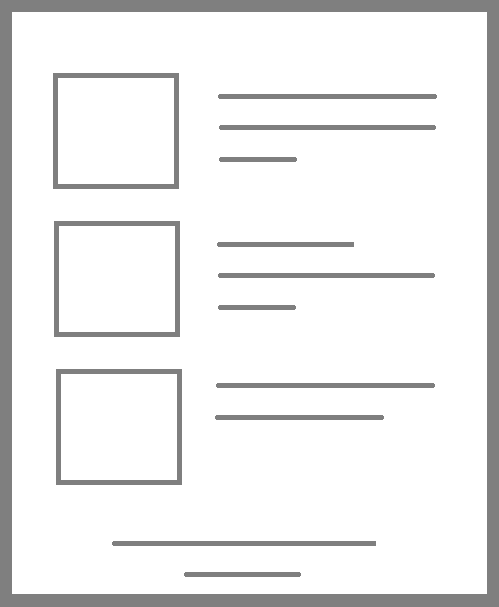
\includegraphics[height=10cm]{besoins/rendu}
\end{center}
\caption{Rendu attendu}
\end{figure}

\subsection{Sous-partie 2}

Bla

\newpage

\section{Développement}

Intro

\subsection{Tâches}

Bla\\


%tableau à taille fixée sur certaines colonnes (param sur la ligne \begin{tabularx}, voir wiki pour plus d'info sur la syntaxe
\begin{figure}[!h]
\begin{center}
\begin{tabularx}{17cm}{|c|p{6cm}|X|}
  \hline
  Priorité & Nom & Raison\\
  \hline
  1 & Tache 1 & Doit être vérifié en premier car sinon [...] \tabularnewline
  2 & Tache 2 & On doit pouvoir [...] \tabularnewline
  3 & Tache 3 & Comme les principales fonctionnalités permettant de tester sont opérationnelles, nous pouvons passer à cette tâche. \tabularnewline
  4 & Tache 4 & Parce que [...] \tabularnewline
  5 & Tache 5 & La tache 5 fait partie des principales [...]. \tabularnewline
  6 & Tache 6 & Dernière fonctionnalité essentielle à mettre en place. \tabularnewline
  7 & Tache 7 & Non-essentiel, mais apporterait un plus au projet. \tabularnewline
  8 & Tache 8 & Non-essentiel, mais apporterait un plus au projet. \tabularnewline
  \hline
\end{tabularx}
\end{center}
\caption{Tableau récapitulatif des tâches}
\end{figure}

\subsection{Tests}

Bla\\

\begin{figure}[!h]
\begin{center}
\begin{tabularx}{17cm}{|p{6cm}|X|}
  \hline
  Fonctionnalité & Test\\
  \hline
  Fonction 1 & Quand [...], vérifier [...]. \tabularnewline
  & Et quand [...], vérifier [...]. \tabularnewline
  Fonction 2 & Vérifier [...]. \tabularnewline
  Fonction 3 & Vérifier [...]. \tabularnewline
  Fonction 4 & Avoir [...]. \tabularnewline
  Fonction 5 & Accéder à [...]. \tabularnewline
   & Vérifier que [...]. \tabularnewline
  Fonction 6 & Accéder à [...]. \tabularnewline
   & Et vérifier [...]. \tabularnewline
  Fonction 7 & Installer [...]. \tabularnewline
   & Vérifier [...]. \tabularnewline
  Fonction 8 & Compter [...]. \tabularnewline
  \hline
\end{tabularx}
\end{center}
\caption{Tableau récapitulatif des tests}
\end{figure}
\fi